\documentclass[1p]{elsarticle_modified}
%\bibliographystyle{elsarticle-num}

%\usepackage[colorlinks]{hyperref}
%\usepackage{abbrmath_seonhwa} %\Abb, \Ascr, \Acal ,\Abf, \Afrak
\usepackage{amsfonts}
\usepackage{amssymb}
\usepackage{amsmath}
\usepackage{amsthm}
\usepackage{scalefnt}
\usepackage{amsbsy}
\usepackage{kotex}
\usepackage{caption}
\usepackage{subfig}
\usepackage{color}
\usepackage{graphicx}
\usepackage{xcolor} %% white, black, red, green, blue, cyan, magenta, yellow
\usepackage{float}
\usepackage{setspace}
\usepackage{hyperref}

\usepackage{tikz}
\usetikzlibrary{arrows}

\usepackage{multirow}
\usepackage{array} % fixed length table
\usepackage{hhline}

%%%%%%%%%%%%%%%%%%%%%
\makeatletter
\renewcommand*\env@matrix[1][\arraystretch]{%
	\edef\arraystretch{#1}%
	\hskip -\arraycolsep
	\let\@ifnextchar\new@ifnextchar
	\array{*\c@MaxMatrixCols c}}
\makeatother %https://tex.stackexchange.com/questions/14071/how-can-i-increase-the-line-spacing-in-a-matrix
%%%%%%%%%%%%%%%

\usepackage[normalem]{ulem}

\newcommand{\msout}[1]{\ifmmode\text{\sout{\ensuremath{#1}}}\else\sout{#1}\fi}
%SOURCE: \msout is \stkout macro in https://tex.stackexchange.com/questions/20609/strikeout-in-math-mode

\newcommand{\cancel}[1]{
	\ifmmode
	{\color{red}\msout{#1}}
	\else
	{\color{red}\sout{#1}}
	\fi
}

\newcommand{\add}[1]{
	{\color{blue}\uwave{#1}}
}

\newcommand{\replace}[2]{
	\ifmmode
	{\color{red}\msout{#1}}{\color{blue}\uwave{#2}}
	\else
	{\color{red}\sout{#1}}{\color{blue}\uwave{#2}}
	\fi
}

\newcommand{\Sol}{\mathcal{S}} %segment
\newcommand{\D}{D} %diagram
\newcommand{\A}{\mathcal{A}} %arc


%%%%%%%%%%%%%%%%%%%%%%%%%%%%%5 test

\def\sl{\operatorname{\textup{SL}}(2,\Cbb)}
\def\psl{\operatorname{\textup{PSL}}(2,\Cbb)}
\def\quan{\mkern 1mu \triangleright \mkern 1mu}

\theoremstyle{definition}
\newtheorem{thm}{Theorem}[section]
\newtheorem{prop}[thm]{Proposition}
\newtheorem{lem}[thm]{Lemma}
\newtheorem{ques}[thm]{Question}
\newtheorem{cor}[thm]{Corollary}
\newtheorem{defn}[thm]{Definition}
\newtheorem{exam}[thm]{Example}
\newtheorem{rmk}[thm]{Remark}
\newtheorem{alg}[thm]{Algorithm}

\newcommand{\I}{\sqrt{-1}}
\begin{document}

%\begin{frontmatter}
%
%\title{Boundary parabolic representations of knots up to 8 crossings}
%
%%% Group authors per affiliation:
%\author{Yunhi Cho} 
%\address{Department of Mathematics, University of Seoul, Seoul, Korea}
%\ead{yhcho@uos.ac.kr}
%
%
%\author{Seonhwa Kim} %\fnref{s_kim}}
%\address{Center for Geometry and Physics, Institute for Basic Science, Pohang, 37673, Korea}
%\ead{ryeona17@ibs.re.kr}
%
%\author{Hyuk Kim}
%\address{Department of Mathematical Sciences, Seoul National University, Seoul 08826, Korea}
%\ead{hyukkim@snu.ac.kr}
%
%\author{Seokbeom Yoon}
%\address{Department of Mathematical Sciences, Seoul National University, Seoul, 08826,  Korea}
%\ead{sbyoon15@snu.ac.kr}
%
%\begin{abstract}
%We find all boundary parabolic representation of knots up to 8 crossings.
%
%\end{abstract}
%\begin{keyword}
%    \MSC[2010] 57M25 
%\end{keyword}
%
%\end{frontmatter}

%\linenumbers
%\tableofcontents
%
\newcommand\colored[1]{\textcolor{white}{\rule[-0.35ex]{0.8em}{1.4ex}}\kern-0.8em\color{red} #1}%
%\newcommand\colored[1]{\textcolor{white}{ #1}\kern-2.17ex	\textcolor{white}{ #1}\kern-1.81ex	\textcolor{white}{ #1}\kern-2.15ex\color{red}#1	}

{\Large $\underline{12a_{0574}~(K12a_{0574})}$}

\setlength{\tabcolsep}{10pt}
\renewcommand{\arraystretch}{1.6}
\vspace{1cm}\begin{tabular}{m{100pt}>{\centering\arraybackslash}m{274pt}}
\multirow{5}{120pt}{
	\centering
	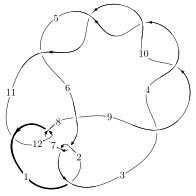
\includegraphics[width=112pt]{../../../GIT/diagram.site/Diagrams/png/1375_12a_0574.png}\\
\ \ \ A knot diagram\footnotemark}&
\allowdisplaybreaks
\textbf{Linearized knot diagam} \\
\cline{2-2}
 &
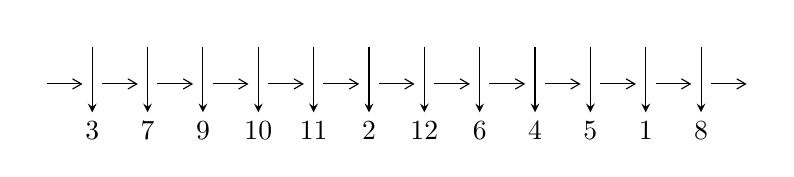
\begin{tikzpicture}[x=20pt, y=17pt]
	% nodes
	\node (C0) at (0, 0) {};
	\node (C1) at (1, 0) {};
	\node (C1U) at (1, +1) {};
	\node (C1D) at (1, -1) {3};

	\node (C2) at (2, 0) {};
	\node (C2U) at (2, +1) {};
	\node (C2D) at (2, -1) {7};

	\node (C3) at (3, 0) {};
	\node (C3U) at (3, +1) {};
	\node (C3D) at (3, -1) {9};

	\node (C4) at (4, 0) {};
	\node (C4U) at (4, +1) {};
	\node (C4D) at (4, -1) {10};

	\node (C5) at (5, 0) {};
	\node (C5U) at (5, +1) {};
	\node (C5D) at (5, -1) {11};

	\node (C6) at (6, 0) {};
	\node (C6U) at (6, +1) {};
	\node (C6D) at (6, -1) {2};

	\node (C7) at (7, 0) {};
	\node (C7U) at (7, +1) {};
	\node (C7D) at (7, -1) {12};

	\node (C8) at (8, 0) {};
	\node (C8U) at (8, +1) {};
	\node (C8D) at (8, -1) {6};

	\node (C9) at (9, 0) {};
	\node (C9U) at (9, +1) {};
	\node (C9D) at (9, -1) {4};

	\node (C10) at (10, 0) {};
	\node (C10U) at (10, +1) {};
	\node (C10D) at (10, -1) {5};

	\node (C11) at (11, 0) {};
	\node (C11U) at (11, +1) {};
	\node (C11D) at (11, -1) {1};

	\node (C12) at (12, 0) {};
	\node (C12U) at (12, +1) {};
	\node (C12D) at (12, -1) {8};
	\node (C13) at (13, 0) {};

	% arrows
	\draw[->,>={angle 60}]
	(C0) edge (C1) (C1) edge (C2) (C2) edge (C3) (C3) edge (C4) (C4) edge (C5) (C5) edge (C6) (C6) edge (C7) (C7) edge (C8) (C8) edge (C9) (C9) edge (C10) (C10) edge (C11) (C11) edge (C12) (C12) edge (C13) ;	\draw[->,>=stealth]
	(C1U) edge (C1D) (C2U) edge (C2D) (C3U) edge (C3D) (C4U) edge (C4D) (C5U) edge (C5D) (C6U) edge (C6D) (C7U) edge (C7D) (C8U) edge (C8D) (C9U) edge (C9D) (C10U) edge (C10D) (C11U) edge (C11D) (C12U) edge (C12D) ;
	\end{tikzpicture} \\
\hhline{~~} \\& 
\textbf{Solving Sequence} \\ \cline{2-2} 
 &
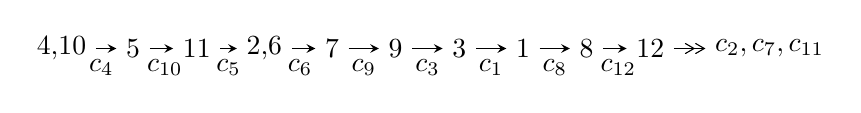
\begin{tikzpicture}[x=23pt, y=7pt]
	% node
	\node (A0) at (-1/8, 0) {4,10};
	\node (A1) at (1, 0) {5};
	\node (A2) at (2, 0) {11};
	\node (A3) at (49/16, 0) {2,6};
	\node (A4) at (33/8, 0) {7};
	\node (A5) at (41/8, 0) {9};
	\node (A6) at (49/8, 0) {3};
	\node (A7) at (57/8, 0) {1};
	\node (A8) at (65/8, 0) {8};
	\node (A9) at (73/8, 0) {12};
	\node (C1) at (1/2, -1) {$c_{4}$};
	\node (C2) at (3/2, -1) {$c_{10}$};
	\node (C3) at (5/2, -1) {$c_{5}$};
	\node (C4) at (29/8, -1) {$c_{6}$};
	\node (C5) at (37/8, -1) {$c_{9}$};
	\node (C6) at (45/8, -1) {$c_{3}$};
	\node (C7) at (53/8, -1) {$c_{1}$};
	\node (C8) at (61/8, -1) {$c_{8}$};
	\node (C9) at (69/8, -1) {$c_{12}$};
	\node (A10) at (11, 0) {$c_{2},c_{7},c_{11}$};

	% edge
	\draw[->,>=stealth]	
	(A0) edge (A1) (A1) edge (A2) (A2) edge (A3) (A3) edge (A4) (A4) edge (A5) (A5) edge (A6) (A6) edge (A7) (A7) edge (A8) (A8) edge (A9) ;
	\draw[->>,>={angle 60}]	
	(A9) edge (A10);
\end{tikzpicture} \\ 

\end{tabular} \\

\footnotetext{
The image of knot diagram is generated by the software ``\textbf{Draw programme}" developed by Andrew Bartholomew(\url{http://www.layer8.co.uk/maths/draw/index.htm\#Running-draw}), where we modified some parts for our purpose(\url{https://github.com/CATsTAILs/LinksPainter}).
}\phantom \\ \newline 
\centering \textbf{Ideals for irreducible components\footnotemark of $X_{\text{par}}$} 
 
\begin{align*}
I^u_{1}&=\langle 
4 u^{24}-5 u^{23}+\cdots+b+5,\;5 u^{24}-7 u^{23}+\cdots+2 a+4,\;u^{25}-3 u^{24}+\cdots+9 u^2-2\rangle \\
I^u_{2}&=\langle 
u^{17} a- u^{17}+\cdots+b+a,\;2 u^{17} a+2 u^{17}+\cdots+a^2+2,\;u^{18}+2 u^{17}+\cdots+u+1\rangle \\
I^u_{3}&=\langle 
b- u+1,\;3 a-2 u+3,\;u^2-3\rangle \\
I^u_{4}&=\langle 
b,\;a+1,\;u+1\rangle \\
I^u_{5}&=\langle 
b+2,\;a+1,\;u-1\rangle \\
I^u_{6}&=\langle 
b+1,\;a,\;u-1\rangle \\
I^u_{7}&=\langle 
b+1,\;a+1,\;u-1\rangle \\
\\
I^v_{1}&=\langle 
a,\;b+1,\;v+1\rangle \\
\end{align*}
\raggedright * 8 irreducible components of $\dim_{\mathbb{C}}=0$, with total 68 representations.\\
\footnotetext{All coefficients of polynomials are rational numbers. But the coefficients are sometimes approximated in decimal forms when there is not enough margin.}
\newpage
\renewcommand{\arraystretch}{1}
\centering \section*{I. $I^u_{1}= \langle 4 u^{24}-5 u^{23}+\cdots+b+5,\;5 u^{24}-7 u^{23}+\cdots+2 a+4,\;u^{25}-3 u^{24}+\cdots+9 u^2-2 \rangle$}
\flushleft \textbf{(i) Arc colorings}\\
\begin{tabular}{m{7pt} m{180pt} m{7pt} m{180pt} }
\flushright $a_{4}=$&$\begin{pmatrix}1\\0\end{pmatrix}$ \\
\flushright $a_{10}=$&$\begin{pmatrix}0\\u\end{pmatrix}$ \\
\flushright $a_{5}=$&$\begin{pmatrix}1\\u^2\end{pmatrix}$ \\
\flushright $a_{11}=$&$\begin{pmatrix}- u\\- u^3+u\end{pmatrix}$ \\
\flushright $a_{2}=$&$\begin{pmatrix}-\frac{5}{2} u^{24}+\frac{7}{2} u^{23}+\cdots-\frac{3}{2} u-2\\-4 u^{24}+5 u^{23}+\cdots-3 u-5\end{pmatrix}$ \\
\flushright $a_{6}=$&$\begin{pmatrix}- u^2+1\\- u^4+2 u^2\end{pmatrix}$ \\
\flushright $a_{7}=$&$\begin{pmatrix}-\frac{5}{2} u^{24}+\frac{7}{2} u^{23}+\cdots-\frac{3}{2} u-2\\-3 u^{24}+4 u^{23}+\cdots-2 u-3\end{pmatrix}$ \\
\flushright $a_{9}=$&$\begin{pmatrix}u\\u\end{pmatrix}$ \\
\flushright $a_{3}=$&$\begin{pmatrix}- u^2+1\\- u^2\end{pmatrix}$ \\
\flushright $a_{1}=$&$\begin{pmatrix}-\frac{9}{2} u^{24}+\frac{13}{2} u^{23}+\cdots-\frac{7}{2} u-5\\-7 u^{24}+9 u^{23}+\cdots-5 u-9\end{pmatrix}$ \\
\flushright $a_{8}=$&$\begin{pmatrix}- u^7+4 u^5-4 u^3+2 u\\- u^9+5 u^7-7 u^5+2 u^3+u\end{pmatrix}$ \\
\flushright $a_{12}=$&$\begin{pmatrix}\frac{5}{2} u^{24}-\frac{7}{2} u^{23}+\cdots+\frac{1}{2} u+3\\4 u^{24}-5 u^{23}+\cdots+4 u+5\end{pmatrix}$\\&\end{tabular}
\flushleft \textbf{(ii) Obstruction class $= -1$}\\~\\
\flushleft \textbf{(iii) Cusp Shapes $= 8 u^{24}-8 u^{23}-118 u^{22}+104 u^{21}+738 u^{20}-568 u^{19}-2532 u^{18}+1728 u^{17}+5122 u^{16}-3322 u^{15}-6024 u^{14}+4356 u^{13}+3552 u^{12}-3876 u^{11}-116 u^{10}+1936 u^9-1222 u^8-156 u^7+670 u^6-304 u^5-22 u^4+112 u^3-56 u^2+16 u-4$}\\~\\
\newpage\renewcommand{\arraystretch}{1}
\flushleft \textbf{(iv) u-Polynomials at the component}\newline \\
\begin{tabular}{m{50pt}|m{274pt}}
Crossings & \hspace{64pt}u-Polynomials at each crossing \\
\hline $$\begin{aligned}c_{1},c_{11}\end{aligned}$$&$\begin{aligned}
&u^{25}+11 u^{24}+\cdots+16 u+1
\end{aligned}$\\
\hline $$\begin{aligned}c_{2},c_{6},c_{7}\\c_{12}\end{aligned}$$&$\begin{aligned}
&u^{25}- u^{24}+\cdots-2 u-1
\end{aligned}$\\
\hline $$\begin{aligned}c_{3},c_{4},c_{5}\\c_{9},c_{10}\end{aligned}$$&$\begin{aligned}
&u^{25}-3 u^{24}+\cdots+9 u^2-2
\end{aligned}$\\
\hline $$\begin{aligned}c_{8}\end{aligned}$$&$\begin{aligned}
&u^{25}-15 u^{24}+\cdots-272 u+142
\end{aligned}$\\
\hline
\end{tabular}\\~\\
\newpage\renewcommand{\arraystretch}{1}
\flushleft \textbf{(v) Riley Polynomials at the component}\newline \\
\begin{tabular}{m{50pt}|m{274pt}}
Crossings & \hspace{64pt}Riley Polynomials at each crossing \\
\hline $$\begin{aligned}c_{1},c_{11}\end{aligned}$$&$\begin{aligned}
&y^{25}+13 y^{24}+\cdots+88 y-1
\end{aligned}$\\
\hline $$\begin{aligned}c_{2},c_{6},c_{7}\\c_{12}\end{aligned}$$&$\begin{aligned}
&y^{25}-11 y^{24}+\cdots+16 y-1
\end{aligned}$\\
\hline $$\begin{aligned}c_{3},c_{4},c_{5}\\c_{9},c_{10}\end{aligned}$$&$\begin{aligned}
&y^{25}-33 y^{24}+\cdots+36 y-4
\end{aligned}$\\
\hline $$\begin{aligned}c_{8}\end{aligned}$$&$\begin{aligned}
&y^{25}-9 y^{24}+\cdots+269092 y-20164
\end{aligned}$\\
\hline
\end{tabular}\\~\\
\newpage\flushleft \textbf{(vi) Complex Volumes and Cusp Shapes}
$$\begin{array}{c|c|c}  
\text{Solutions to }I^u_{1}& \I (\text{vol} + \sqrt{-1}CS) & \text{Cusp shape}\\
 \hline 
\begin{aligned}
u &= -1.014520 + 0.347002 I \\
a &= -0.043435 + 0.313283 I \\
b &= \phantom{-}1.26937 + 1.85429 I\end{aligned}
 & -4.53390 + 11.98000 I & -18.3056 - 9.4054 I \\ \hline\begin{aligned}
u &= -1.014520 - 0.347002 I \\
a &= -0.043435 - 0.313283 I \\
b &= \phantom{-}1.26937 - 1.85429 I\end{aligned}
 & -4.53390 - 11.98000 I & -18.3056 + 9.4054 I \\ \hline\begin{aligned}
u &= -0.875840 + 0.298355 I \\
a &= \phantom{-}0.324656 + 0.199831 I \\
b &= -0.824925 - 0.525750 I\end{aligned}
 & -0.08743 + 1.64240 I & -12.36047 - 1.45966 I \\ \hline\begin{aligned}
u &= -0.875840 - 0.298355 I \\
a &= \phantom{-}0.324656 - 0.199831 I \\
b &= -0.824925 + 0.525750 I\end{aligned}
 & -0.08743 - 1.64240 I & -12.36047 + 1.45966 I \\ \hline\begin{aligned}
u &= \phantom{-}1.08434\phantom{ +0.000000I} \\
a &= -0.492978\phantom{ +0.000000I} \\
b &= -0.942393\phantom{ +0.000000I}\end{aligned}
 & -5.05178\phantom{ +0.000000I} & -16.4940\phantom{ +0.000000I} \\ \hline\begin{aligned}
u &= -1.142900 + 0.163650 I \\
a &= -0.760257 - 0.659750 I \\
b &= -1.148230 - 0.116814 I\end{aligned}
 & -6.80316 - 3.32641 I & -19.9139 + 4.3823 I \\ \hline\begin{aligned}
u &= -1.142900 - 0.163650 I \\
a &= -0.760257 + 0.659750 I \\
b &= -1.148230 + 0.116814 I\end{aligned}
 & -6.80316 + 3.32641 I & -19.9139 - 4.3823 I \\ \hline\begin{aligned}
u &= \phantom{-}0.748460 + 0.331609 I \\
a &= \phantom{-}0.182754 - 0.355577 I \\
b &= \phantom{-}0.439503 - 1.224670 I\end{aligned}
 & \phantom{-}0.58577 - 4.17677 I & -12.9289 + 7.8019 I \\ \hline\begin{aligned}
u &= \phantom{-}0.748460 - 0.331609 I \\
a &= \phantom{-}0.182754 + 0.355577 I \\
b &= \phantom{-}0.439503 + 1.224670 I\end{aligned}
 & \phantom{-}0.58577 + 4.17677 I & -12.9289 - 7.8019 I \\ \hline\begin{aligned}
u &= \phantom{-}0.489290 + 0.461642 I \\
a &= \phantom{-}0.494840 - 0.083674 I \\
b &= -1.112620 + 0.488193 I\end{aligned}
 & -1.55633 + 5.36068 I & -15.2414 - 2.7515 I\\
 \hline 
 \end{array}$$\newpage$$\begin{array}{c|c|c}  
\text{Solutions to }I^u_{1}& \I (\text{vol} + \sqrt{-1}CS) & \text{Cusp shape}\\
 \hline 
\begin{aligned}
u &= \phantom{-}0.489290 - 0.461642 I \\
a &= \phantom{-}0.494840 + 0.083674 I \\
b &= -1.112620 - 0.488193 I\end{aligned}
 & -1.55633 - 5.36068 I & -15.2414 + 2.7515 I \\ \hline\begin{aligned}
u &= \phantom{-}0.223404 + 0.580813 I \\
a &= \phantom{-}0.00021 + 2.17964 I \\
b &= -0.147329 - 0.569907 I\end{aligned}
 & -0.71018 - 8.82975 I & -13.3096 + 8.6436 I \\ \hline\begin{aligned}
u &= \phantom{-}0.223404 - 0.580813 I \\
a &= \phantom{-}0.00021 - 2.17964 I \\
b &= -0.147329 + 0.569907 I\end{aligned}
 & -0.71018 + 8.82975 I & -13.3096 - 8.6436 I \\ \hline\begin{aligned}
u &= \phantom{-}0.047295 + 0.535702 I \\
a &= \phantom{-}0.79115 - 1.42217 I \\
b &= \phantom{-}0.192529 + 0.279886 I\end{aligned}
 & \phantom{-}2.69786 + 1.19945 I & -6.93738 - 2.54623 I \\ \hline\begin{aligned}
u &= \phantom{-}0.047295 - 0.535702 I \\
a &= \phantom{-}0.79115 + 1.42217 I \\
b &= \phantom{-}0.192529 - 0.279886 I\end{aligned}
 & \phantom{-}2.69786 - 1.19945 I & -6.93738 + 2.54623 I \\ \hline\begin{aligned}
u &= -1.63846 + 0.04838 I \\
a &= -0.24414 + 2.30889 I \\
b &= -0.31656 + 2.94869 I\end{aligned}
 & -7.64782 + 5.42310 I & -15.0279 - 5.6441 I \\ \hline\begin{aligned}
u &= -1.63846 - 0.04838 I \\
a &= -0.24414 - 2.30889 I \\
b &= -0.31656 - 2.94869 I\end{aligned}
 & -7.64782 - 5.42310 I & -15.0279 + 5.6441 I \\ \hline\begin{aligned}
u &= -0.337545\phantom{ +0.000000I} \\
a &= \phantom{-}0.668217\phantom{ +0.000000I} \\
b &= -0.205875\phantom{ +0.000000I}\end{aligned}
 & -0.538410\phantom{ +0.000000I} & -18.2630\phantom{ +0.000000I} \\ \hline\begin{aligned}
u &= \phantom{-}1.68786 + 0.06949 I \\
a &= -1.26126 + 1.27240 I \\
b &= -2.17832 + 1.75017 I\end{aligned}
 & -9.13866 - 3.01203 I & -13.72954 + 0. I\phantom{ +0.000000I} \\ \hline\begin{aligned}
u &= \phantom{-}1.68786 - 0.06949 I \\
a &= -1.26126 - 1.27240 I \\
b &= -2.17832 - 1.75017 I\end{aligned}
 & -9.13866 + 3.01203 I & -13.72954 + 0. I\phantom{ +0.000000I}\\
 \hline 
 \end{array}$$\newpage$$\begin{array}{c|c|c}  
\text{Solutions to }I^u_{1}& \I (\text{vol} + \sqrt{-1}CS) & \text{Cusp shape}\\
 \hline 
\begin{aligned}
u &= \phantom{-}1.72244 + 0.09263 I \\
a &= \phantom{-}1.48000 - 2.81178 I \\
b &= \phantom{-}2.64308 - 3.71258 I\end{aligned}
 & -14.2211 - 13.7690 I & -19.5082 + 7.8820 I \\ \hline\begin{aligned}
u &= \phantom{-}1.72244 - 0.09263 I \\
a &= \phantom{-}1.48000 + 2.81178 I \\
b &= \phantom{-}2.64308 + 3.71258 I\end{aligned}
 & -14.2211 + 13.7690 I & -19.5082 - 7.8820 I \\ \hline\begin{aligned}
u &= -1.74758\phantom{ +0.000000I} \\
a &= -1.18512\phantom{ +0.000000I} \\
b &= -1.50038\phantom{ +0.000000I}\end{aligned}
 & -15.2938\phantom{ +0.000000I} & -14.4450\phantom{ +0.000000I} \\ \hline\begin{aligned}
u &= \phantom{-}1.75336 + 0.03699 I \\
a &= -0.959572 - 0.248462 I \\
b &= -0.992169 - 0.771791 I\end{aligned}
 & -17.2303 + 2.5055 I & -21.1359 - 5.5116 I \\ \hline\begin{aligned}
u &= \phantom{-}1.75336 - 0.03699 I \\
a &= -0.959572 + 0.248462 I \\
b &= -0.992169 + 0.771791 I\end{aligned}
 & -17.2303 - 2.5055 I & -21.1359 + 5.5116 I\\
 \hline 
 \end{array}$$\newpage\newpage\renewcommand{\arraystretch}{1}
\centering \section*{II. $I^u_{2}= \langle u^{17} a- u^{17}+\cdots+b+a,\;2 u^{17} a+2 u^{17}+\cdots+a^2+2,\;u^{18}+2 u^{17}+\cdots+u+1 \rangle$}
\flushleft \textbf{(i) Arc colorings}\\
\begin{tabular}{m{7pt} m{180pt} m{7pt} m{180pt} }
\flushright $a_{4}=$&$\begin{pmatrix}1\\0\end{pmatrix}$ \\
\flushright $a_{10}=$&$\begin{pmatrix}0\\u\end{pmatrix}$ \\
\flushright $a_{5}=$&$\begin{pmatrix}1\\u^2\end{pmatrix}$ \\
\flushright $a_{11}=$&$\begin{pmatrix}- u\\- u^3+u\end{pmatrix}$ \\
\flushright $a_{2}=$&$\begin{pmatrix}a\\- u^{17} a+u^{17}+\cdots- a+u\end{pmatrix}$ \\
\flushright $a_{6}=$&$\begin{pmatrix}- u^2+1\\- u^4+2 u^2\end{pmatrix}$ \\
\flushright $a_{7}=$&$\begin{pmatrix}a\\u^{17} a- u^{17}+\cdots+a- u\end{pmatrix}$ \\
\flushright $a_{9}=$&$\begin{pmatrix}u\\u\end{pmatrix}$ \\
\flushright $a_{3}=$&$\begin{pmatrix}- u^2+1\\- u^2\end{pmatrix}$ \\
\flushright $a_{1}=$&$\begin{pmatrix}- u^{17} a+11 u^{15} a+\cdots+a-1\\-2 u^{17} a+u^{17}+\cdots- a+u\end{pmatrix}$ \\
\flushright $a_{8}=$&$\begin{pmatrix}- u^7+4 u^5-4 u^3+2 u\\- u^9+5 u^7-7 u^5+2 u^3+u\end{pmatrix}$ \\
\flushright $a_{12}=$&$\begin{pmatrix}- u^{13}- u^{11} a+\cdots+a-1\\u^{17} a+u^{17}+\cdots+2 u^2+a\end{pmatrix}$\\&\end{tabular}
\flushleft \textbf{(ii) Obstruction class $= -1$}\\~\\
\flushleft \textbf{(iii) Cusp Shapes $= 4 u^{15}-40 u^{13}+152 u^{11}+4 u^{10}-272 u^9-28 u^8+232 u^7+64 u^6-84 u^5-52 u^4+12 u^2+4 u-14$}\\~\\
\newpage\renewcommand{\arraystretch}{1}
\flushleft \textbf{(iv) u-Polynomials at the component}\newline \\
\begin{tabular}{m{50pt}|m{274pt}}
Crossings & \hspace{64pt}u-Polynomials at each crossing \\
\hline $$\begin{aligned}c_{1},c_{11}\end{aligned}$$&$\begin{aligned}
&u^{36}+20 u^{35}+\cdots+66 u+9
\end{aligned}$\\
\hline $$\begin{aligned}c_{2},c_{6},c_{7}\\c_{12}\end{aligned}$$&$\begin{aligned}
&u^{36}-10 u^{34}+\cdots+11 u^2-3
\end{aligned}$\\
\hline $$\begin{aligned}c_{3},c_{4},c_{5}\\c_{9},c_{10}\end{aligned}$$&$\begin{aligned}
&(u^{18}+2 u^{17}+\cdots+u+1)^{2}
\end{aligned}$\\
\hline $$\begin{aligned}c_{8}\end{aligned}$$&$\begin{aligned}
&(u^{18}+4 u^{17}+\cdots+5 u-1)^{2}
\end{aligned}$\\
\hline
\end{tabular}\\~\\
\newpage\renewcommand{\arraystretch}{1}
\flushleft \textbf{(v) Riley Polynomials at the component}\newline \\
\begin{tabular}{m{50pt}|m{274pt}}
Crossings & \hspace{64pt}Riley Polynomials at each crossing \\
\hline $$\begin{aligned}c_{1},c_{11}\end{aligned}$$&$\begin{aligned}
&y^{36}-8 y^{35}+\cdots+198 y+81
\end{aligned}$\\
\hline $$\begin{aligned}c_{2},c_{6},c_{7}\\c_{12}\end{aligned}$$&$\begin{aligned}
&y^{36}-20 y^{35}+\cdots-66 y+9
\end{aligned}$\\
\hline $$\begin{aligned}c_{3},c_{4},c_{5}\\c_{9},c_{10}\end{aligned}$$&$\begin{aligned}
&(y^{18}-24 y^{17}+\cdots+3 y+1)^{2}
\end{aligned}$\\
\hline $$\begin{aligned}c_{8}\end{aligned}$$&$\begin{aligned}
&(y^{18}+22 y^{16}+\cdots-65 y+1)^{2}
\end{aligned}$\\
\hline
\end{tabular}\\~\\
\newpage\flushleft \textbf{(vi) Complex Volumes and Cusp Shapes}
$$\begin{array}{c|c|c}  
\text{Solutions to }I^u_{2}& \I (\text{vol} + \sqrt{-1}CS) & \text{Cusp shape}\\
 \hline 
\begin{aligned}
u &= -0.972680 + 0.237177 I \\
a &= -1.129940 - 0.718306 I \\
b &= -1.113160 + 0.114624 I\end{aligned}
 & -6.99539 + 3.19755 I & -20.6137 - 5.3239 I \\ \hline\begin{aligned}
u &= -0.972680 + 0.237177 I \\
a &= \phantom{-}0.005899 + 0.226891 I \\
b &= \phantom{-}0.94715 + 2.42519 I\end{aligned}
 & -6.99539 + 3.19755 I & -20.6137 - 5.3239 I \\ \hline\begin{aligned}
u &= -0.972680 - 0.237177 I \\
a &= -1.129940 + 0.718306 I \\
b &= -1.113160 - 0.114624 I\end{aligned}
 & -6.99539 - 3.19755 I & -20.6137 + 5.3239 I \\ \hline\begin{aligned}
u &= -0.972680 - 0.237177 I \\
a &= \phantom{-}0.005899 - 0.226891 I \\
b &= \phantom{-}0.94715 - 2.42519 I\end{aligned}
 & -6.99539 - 3.19755 I & -20.6137 + 5.3239 I \\ \hline\begin{aligned}
u &= \phantom{-}0.965445 + 0.329507 I \\
a &= \phantom{-}0.319004 - 0.279303 I \\
b &= -0.711465 + 0.510542 I\end{aligned}
 & -1.96003 - 6.64718 I & -15.2451 + 6.1969 I \\ \hline\begin{aligned}
u &= \phantom{-}0.965445 + 0.329507 I \\
a &= -0.001264 - 0.306149 I \\
b &= \phantom{-}1.05963 - 1.87946 I\end{aligned}
 & -1.96003 - 6.64718 I & -15.2451 + 6.1969 I \\ \hline\begin{aligned}
u &= \phantom{-}0.965445 - 0.329507 I \\
a &= \phantom{-}0.319004 + 0.279303 I \\
b &= -0.711465 - 0.510542 I\end{aligned}
 & -1.96003 + 6.64718 I & -15.2451 - 6.1969 I \\ \hline\begin{aligned}
u &= \phantom{-}0.965445 - 0.329507 I \\
a &= -0.001264 + 0.306149 I \\
b &= \phantom{-}1.05963 + 1.87946 I\end{aligned}
 & -1.96003 + 6.64718 I & -15.2451 - 6.1969 I \\ \hline\begin{aligned}
u &= \phantom{-}0.884294\phantom{ +0.000000I} \\
a &= -1.43019\phantom{ +0.000000I} \\
b &= -0.962086\phantom{ +0.000000I}\end{aligned}
 & -5.00473\phantom{ +0.000000I} & -16.9870\phantom{ +0.000000I} \\ \hline\begin{aligned}
u &= \phantom{-}0.884294\phantom{ +0.000000I} \\
a &= \phantom{-}0.144030\phantom{ +0.000000I} \\
b &= -1.72715\phantom{ +0.000000I}\end{aligned}
 & -5.00473\phantom{ +0.000000I} & -16.9870\phantom{ +0.000000I}\\
 \hline 
 \end{array}$$\newpage$$\begin{array}{c|c|c}  
\text{Solutions to }I^u_{2}& \I (\text{vol} + \sqrt{-1}CS) & \text{Cusp shape}\\
 \hline 
\begin{aligned}
u &= -0.572262 + 0.347341 I \\
a &= \phantom{-}0.345746 + 0.427514 I \\
b &= \phantom{-}0.323982 + 0.688753 I\end{aligned}
 & \phantom{-}0.205439 - 0.564924 I & -12.70794 - 1.84066 I \\ \hline\begin{aligned}
u &= -0.572262 + 0.347341 I \\
a &= \phantom{-}0.448687 + 0.081566 I \\
b &= -0.979928 - 0.500327 I\end{aligned}
 & \phantom{-}0.205439 - 0.564924 I & -12.70794 - 1.84066 I \\ \hline\begin{aligned}
u &= -0.572262 - 0.347341 I \\
a &= \phantom{-}0.345746 - 0.427514 I \\
b &= \phantom{-}0.323982 - 0.688753 I\end{aligned}
 & \phantom{-}0.205439 + 0.564924 I & -12.70794 + 1.84066 I \\ \hline\begin{aligned}
u &= -0.572262 - 0.347341 I \\
a &= \phantom{-}0.448687 - 0.081566 I \\
b &= -0.979928 + 0.500327 I\end{aligned}
 & \phantom{-}0.205439 + 0.564924 I & -12.70794 + 1.84066 I \\ \hline\begin{aligned}
u &= -0.158501 + 0.549521 I \\
a &= \phantom{-}0.656801 + 1.100770 I \\
b &= \phantom{-}0.342703 - 0.177435 I\end{aligned}
 & \phantom{-}1.49299 + 3.66002 I & -9.51029 - 4.64953 I \\ \hline\begin{aligned}
u &= -0.158501 + 0.549521 I \\
a &= \phantom{-}0.32363 - 2.20170 I \\
b &= -0.075367 + 0.478624 I\end{aligned}
 & \phantom{-}1.49299 + 3.66002 I & -9.51029 - 4.64953 I \\ \hline\begin{aligned}
u &= -0.158501 - 0.549521 I \\
a &= \phantom{-}0.656801 - 1.100770 I \\
b &= \phantom{-}0.342703 + 0.177435 I\end{aligned}
 & \phantom{-}1.49299 - 3.66002 I & -9.51029 + 4.64953 I \\ \hline\begin{aligned}
u &= -0.158501 - 0.549521 I \\
a &= \phantom{-}0.32363 + 2.20170 I \\
b &= -0.075367 - 0.478624 I\end{aligned}
 & \phantom{-}1.49299 - 3.66002 I & -9.51029 + 4.64953 I \\ \hline\begin{aligned}
u &= \phantom{-}0.184698 + 0.383796 I \\
a &= \phantom{-}0.515622 - 0.022033 I \\
b &= -1.164460 + 0.166059 I\end{aligned}
 & -3.44032 - 1.02752 I & -14.6811 + 6.4558 I \\ \hline\begin{aligned}
u &= \phantom{-}0.184698 + 0.383796 I \\
a &= \phantom{-}0.63653 + 3.61007 I \\
b &= -0.227517 - 0.284301 I\end{aligned}
 & -3.44032 - 1.02752 I & -14.6811 + 6.4558 I\\
 \hline 
 \end{array}$$\newpage$$\begin{array}{c|c|c}  
\text{Solutions to }I^u_{2}& \I (\text{vol} + \sqrt{-1}CS) & \text{Cusp shape}\\
 \hline 
\begin{aligned}
u &= \phantom{-}0.184698 - 0.383796 I \\
a &= \phantom{-}0.515622 + 0.022033 I \\
b &= -1.164460 - 0.166059 I\end{aligned}
 & -3.44032 + 1.02752 I & -14.6811 - 6.4558 I \\ \hline\begin{aligned}
u &= \phantom{-}0.184698 - 0.383796 I \\
a &= \phantom{-}0.63653 - 3.61007 I \\
b &= -0.227517 + 0.284301 I\end{aligned}
 & -3.44032 + 1.02752 I & -14.6811 - 6.4558 I \\ \hline\begin{aligned}
u &= \phantom{-}1.62858\phantom{ +0.000000I} \\
a &= -0.74507 + 1.95151 I \\
b &= -1.21459 + 2.49051 I\end{aligned}
 & -7.25470\phantom{ +0.000000I} & -14.0270\phantom{ +0.000000I} \\ \hline\begin{aligned}
u &= \phantom{-}1.62858\phantom{ +0.000000I} \\
a &= -0.74507 - 1.95151 I \\
b &= -1.21459 - 2.49051 I\end{aligned}
 & -7.25470\phantom{ +0.000000I} & -14.0270\phantom{ +0.000000I} \\ \hline\begin{aligned}
u &= -1.70718 + 0.02414 I \\
a &= -0.860242 + 0.085930 I \\
b &= -0.559302 + 0.302376 I\end{aligned}
 & -14.4445 + 0.2735 I & -18.2189 + 1.0708 I \\ \hline\begin{aligned}
u &= -1.70718 + 0.02414 I \\
a &= -1.96468 - 1.25832 I \\
b &= -3.02809 - 1.79960 I\end{aligned}
 & -14.4445 + 0.2735 I & -18.2189 + 1.0708 I \\ \hline\begin{aligned}
u &= -1.70718 - 0.02414 I \\
a &= -0.860242 - 0.085930 I \\
b &= -0.559302 - 0.302376 I\end{aligned}
 & -14.4445 - 0.2735 I & -18.2189 - 1.0708 I \\ \hline\begin{aligned}
u &= -1.70718 - 0.02414 I \\
a &= -1.96468 + 1.25832 I \\
b &= -3.02809 + 1.79960 I\end{aligned}
 & -14.4445 - 0.2735 I & -18.2189 - 1.0708 I \\ \hline\begin{aligned}
u &= -1.70822 + 0.08549 I \\
a &= -1.22072 - 1.11193 I \\
b &= -2.18354 - 1.58992 I\end{aligned}
 & -11.40320 + 8.29410 I & -16.5396 - 4.6645 I \\ \hline\begin{aligned}
u &= -1.70822 + 0.08549 I \\
a &= \phantom{-}1.12540 + 2.95401 I \\
b &= \phantom{-}2.04448 + 3.93426 I\end{aligned}
 & -11.40320 + 8.29410 I & -16.5396 - 4.6645 I\\
 \hline 
 \end{array}$$\newpage$$\begin{array}{c|c|c}  
\text{Solutions to }I^u_{2}& \I (\text{vol} + \sqrt{-1}CS) & \text{Cusp shape}\\
 \hline 
\begin{aligned}
u &= -1.70822 - 0.08549 I \\
a &= -1.22072 + 1.11193 I \\
b &= -2.18354 + 1.58992 I\end{aligned}
 & -11.40320 - 8.29410 I & -16.5396 + 4.6645 I \\ \hline\begin{aligned}
u &= -1.70822 - 0.08549 I \\
a &= \phantom{-}1.12540 - 2.95401 I \\
b &= \phantom{-}2.04448 - 3.93426 I\end{aligned}
 & -11.40320 - 8.29410 I & -16.5396 + 4.6645 I \\ \hline\begin{aligned}
u &= \phantom{-}1.71227 + 0.06112 I \\
a &= -0.814985 - 0.187785 I \\
b &= -0.451319 - 0.694586 I\end{aligned}
 & -16.5429 - 4.3884 I & -20.9761 + 3.5533 I \\ \hline\begin{aligned}
u &= \phantom{-}1.71227 + 0.06112 I \\
a &= \phantom{-}1.00266 - 3.75542 I \\
b &= \phantom{-}1.83542 - 5.24315 I\end{aligned}
 & -16.5429 - 4.3884 I & -20.9761 + 3.5533 I \\ \hline\begin{aligned}
u &= \phantom{-}1.71227 - 0.06112 I \\
a &= -0.814985 + 0.187785 I \\
b &= -0.451319 + 0.694586 I\end{aligned}
 & -16.5429 + 4.3884 I & -20.9761 - 3.5533 I \\ \hline\begin{aligned}
u &= \phantom{-}1.71227 - 0.06112 I \\
a &= \phantom{-}1.00266 + 3.75542 I \\
b &= \phantom{-}1.83542 + 5.24315 I\end{aligned}
 & -16.5429 + 4.3884 I & -20.9761 - 3.5533 I\\
 \hline 
 \end{array}$$\newpage\newpage\renewcommand{\arraystretch}{1}
\centering \section*{III. $I^u_{3}= \langle b- u+1,\;3 a-2 u+3,\;u^2-3 \rangle$}
\flushleft \textbf{(i) Arc colorings}\\
\begin{tabular}{m{7pt} m{180pt} m{7pt} m{180pt} }
\flushright $a_{4}=$&$\begin{pmatrix}1\\0\end{pmatrix}$ \\
\flushright $a_{10}=$&$\begin{pmatrix}0\\u\end{pmatrix}$ \\
\flushright $a_{5}=$&$\begin{pmatrix}1\\3\end{pmatrix}$ \\
\flushright $a_{11}=$&$\begin{pmatrix}- u\\-2 u\end{pmatrix}$ \\
\flushright $a_{2}=$&$\begin{pmatrix}\frac{2}{3} u-1\\u-1\end{pmatrix}$ \\
\flushright $a_{6}=$&$\begin{pmatrix}-2\\-3\end{pmatrix}$ \\
\flushright $a_{7}=$&$\begin{pmatrix}-\frac{2}{3} u-1\\- u-2\end{pmatrix}$ \\
\flushright $a_{9}=$&$\begin{pmatrix}u\\u\end{pmatrix}$ \\
\flushright $a_{3}=$&$\begin{pmatrix}-2\\-3\end{pmatrix}$ \\
\flushright $a_{1}=$&$\begin{pmatrix}\frac{2}{3} u+1\\u+2\end{pmatrix}$ \\
\flushright $a_{8}=$&$\begin{pmatrix}- u\\-2 u\end{pmatrix}$ \\
\flushright $a_{12}=$&$\begin{pmatrix}-\frac{1}{3} u+1\\- u+2\end{pmatrix}$\\&\end{tabular}
\flushleft \textbf{(ii) Obstruction class $= 1$}\\~\\
\flushleft \textbf{(iii) Cusp Shapes $= -24$}\\~\\
\newpage\renewcommand{\arraystretch}{1}
\flushleft \textbf{(iv) u-Polynomials at the component}\newline \\
\begin{tabular}{m{50pt}|m{274pt}}
Crossings & \hspace{64pt}u-Polynomials at each crossing \\
\hline $$\begin{aligned}c_{1},c_{2},c_{7}\\c_{11}\end{aligned}$$&$\begin{aligned}
&(u-1)^2
\end{aligned}$\\
\hline $$\begin{aligned}c_{3},c_{4},c_{5}\\c_{8},c_{9},c_{10}\end{aligned}$$&$\begin{aligned}
&u^2-3
\end{aligned}$\\
\hline $$\begin{aligned}c_{6},c_{12}\end{aligned}$$&$\begin{aligned}
&(u+1)^2
\end{aligned}$\\
\hline
\end{tabular}\\~\\
\newpage\renewcommand{\arraystretch}{1}
\flushleft \textbf{(v) Riley Polynomials at the component}\newline \\
\begin{tabular}{m{50pt}|m{274pt}}
Crossings & \hspace{64pt}Riley Polynomials at each crossing \\
\hline $$\begin{aligned}c_{1},c_{2},c_{6}\\c_{7},c_{11},c_{12}\end{aligned}$$&$\begin{aligned}
&(y-1)^2
\end{aligned}$\\
\hline $$\begin{aligned}c_{3},c_{4},c_{5}\\c_{8},c_{9},c_{10}\end{aligned}$$&$\begin{aligned}
&(y-3)^2
\end{aligned}$\\
\hline
\end{tabular}\\~\\
\newpage\flushleft \textbf{(vi) Complex Volumes and Cusp Shapes}
$$\begin{array}{c|c|c}  
\text{Solutions to }I^u_{3}& \I (\text{vol} + \sqrt{-1}CS) & \text{Cusp shape}\\
 \hline 
\begin{aligned}
u &= \phantom{-}1.73205\phantom{ +0.000000I} \\
a &= \phantom{-}0.154701\phantom{ +0.000000I} \\
b &= \phantom{-}0.732051\phantom{ +0.000000I}\end{aligned}
 & -16.4493\phantom{ +0.000000I} & -24.0000\phantom{ +0.000000I} \\ \hline\begin{aligned}
u &= -1.73205\phantom{ +0.000000I} \\
a &= -2.15470\phantom{ +0.000000I} \\
b &= -2.73205\phantom{ +0.000000I}\end{aligned}
 & -16.4493\phantom{ +0.000000I} & -24.0000\phantom{ +0.000000I}\\
 \hline 
 \end{array}$$\newpage\newpage\renewcommand{\arraystretch}{1}
\centering \section*{IV. $I^u_{4}= \langle b,\;a+1,\;u+1 \rangle$}
\flushleft \textbf{(i) Arc colorings}\\
\begin{tabular}{m{7pt} m{180pt} m{7pt} m{180pt} }
\flushright $a_{4}=$&$\begin{pmatrix}1\\0\end{pmatrix}$ \\
\flushright $a_{10}=$&$\begin{pmatrix}0\\-1\end{pmatrix}$ \\
\flushright $a_{5}=$&$\begin{pmatrix}1\\1\end{pmatrix}$ \\
\flushright $a_{11}=$&$\begin{pmatrix}1\\0\end{pmatrix}$ \\
\flushright $a_{2}=$&$\begin{pmatrix}-1\\0\end{pmatrix}$ \\
\flushright $a_{6}=$&$\begin{pmatrix}0\\1\end{pmatrix}$ \\
\flushright $a_{7}=$&$\begin{pmatrix}-1\\1\end{pmatrix}$ \\
\flushright $a_{9}=$&$\begin{pmatrix}-1\\-1\end{pmatrix}$ \\
\flushright $a_{3}=$&$\begin{pmatrix}0\\-1\end{pmatrix}$ \\
\flushright $a_{1}=$&$\begin{pmatrix}-1\\1\end{pmatrix}$ \\
\flushright $a_{8}=$&$\begin{pmatrix}-1\\0\end{pmatrix}$ \\
\flushright $a_{12}=$&$\begin{pmatrix}0\\1\end{pmatrix}$\\&\end{tabular}
\flushleft \textbf{(ii) Obstruction class $= 1$}\\~\\
\flushleft \textbf{(iii) Cusp Shapes $= -24$}\\~\\
\newpage\renewcommand{\arraystretch}{1}
\flushleft \textbf{(iv) u-Polynomials at the component}\newline \\
\begin{tabular}{m{50pt}|m{274pt}}
Crossings & \hspace{64pt}u-Polynomials at each crossing \\
\hline $$\begin{aligned}c_{1},c_{6},c_{9}\\c_{10},c_{11},c_{12}\end{aligned}$$&$\begin{aligned}
&u-1
\end{aligned}$\\
\hline $$\begin{aligned}c_{2},c_{3},c_{4}\\c_{5},c_{7},c_{8}\end{aligned}$$&$\begin{aligned}
&u+1
\end{aligned}$\\
\hline
\end{tabular}\\~\\
\newpage\renewcommand{\arraystretch}{1}
\flushleft \textbf{(v) Riley Polynomials at the component}\newline \\
\begin{tabular}{m{50pt}|m{274pt}}
Crossings & \hspace{64pt}Riley Polynomials at each crossing \\
\hline $$\begin{aligned}c_{1},c_{2},c_{3}\\c_{4},c_{5},c_{6}\\c_{7},c_{8},c_{9}\\c_{10},c_{11},c_{12}\end{aligned}$$&$\begin{aligned}
&y-1
\end{aligned}$\\
\hline
\end{tabular}\\~\\
\newpage\flushleft \textbf{(vi) Complex Volumes and Cusp Shapes}
$$\begin{array}{c|c|c}  
\text{Solutions to }I^u_{4}& \I (\text{vol} + \sqrt{-1}CS) & \text{Cusp shape}\\
 \hline 
\begin{aligned}
u &= -1.00000\phantom{ +0.000000I} \\
a &= -1.00000\phantom{ +0.000000I} \\
b &= \phantom{-0.000000 } 0\end{aligned}
 & -6.57974\phantom{ +0.000000I} & -24.0000\phantom{ +0.000000I}\\
 \hline 
 \end{array}$$\newpage\newpage\renewcommand{\arraystretch}{1}
\centering \section*{V. $I^u_{5}= \langle b+2,\;a+1,\;u-1 \rangle$}
\flushleft \textbf{(i) Arc colorings}\\
\begin{tabular}{m{7pt} m{180pt} m{7pt} m{180pt} }
\flushright $a_{4}=$&$\begin{pmatrix}1\\0\end{pmatrix}$ \\
\flushright $a_{10}=$&$\begin{pmatrix}0\\1\end{pmatrix}$ \\
\flushright $a_{5}=$&$\begin{pmatrix}1\\1\end{pmatrix}$ \\
\flushright $a_{11}=$&$\begin{pmatrix}-1\\0\end{pmatrix}$ \\
\flushright $a_{2}=$&$\begin{pmatrix}-1\\-2\end{pmatrix}$ \\
\flushright $a_{6}=$&$\begin{pmatrix}0\\1\end{pmatrix}$ \\
\flushright $a_{7}=$&$\begin{pmatrix}-1\\-1\end{pmatrix}$ \\
\flushright $a_{9}=$&$\begin{pmatrix}1\\1\end{pmatrix}$ \\
\flushright $a_{3}=$&$\begin{pmatrix}0\\-1\end{pmatrix}$ \\
\flushright $a_{1}=$&$\begin{pmatrix}-1\\-1\end{pmatrix}$ \\
\flushright $a_{8}=$&$\begin{pmatrix}1\\0\end{pmatrix}$ \\
\flushright $a_{12}=$&$\begin{pmatrix}-2\\-1\end{pmatrix}$\\&\end{tabular}
\flushleft \textbf{(ii) Obstruction class $= 1$}\\~\\
\flushleft \textbf{(iii) Cusp Shapes $= -24$}\\~\\
\newpage\renewcommand{\arraystretch}{1}
\flushleft \textbf{(iv) u-Polynomials at the component}\newline \\
\begin{tabular}{m{50pt}|m{274pt}}
Crossings & \hspace{64pt}u-Polynomials at each crossing \\
\hline $$\begin{aligned}c_{1},c_{3},c_{4}\\c_{5},c_{6},c_{8}\\c_{11},c_{12}\end{aligned}$$&$\begin{aligned}
&u-1
\end{aligned}$\\
\hline $$\begin{aligned}c_{2},c_{7},c_{9}\\c_{10}\end{aligned}$$&$\begin{aligned}
&u+1
\end{aligned}$\\
\hline
\end{tabular}\\~\\
\newpage\renewcommand{\arraystretch}{1}
\flushleft \textbf{(v) Riley Polynomials at the component}\newline \\
\begin{tabular}{m{50pt}|m{274pt}}
Crossings & \hspace{64pt}Riley Polynomials at each crossing \\
\hline $$\begin{aligned}c_{1},c_{2},c_{3}\\c_{4},c_{5},c_{6}\\c_{7},c_{8},c_{9}\\c_{10},c_{11},c_{12}\end{aligned}$$&$\begin{aligned}
&y-1
\end{aligned}$\\
\hline
\end{tabular}\\~\\
\newpage\flushleft \textbf{(vi) Complex Volumes and Cusp Shapes}
$$\begin{array}{c|c|c}  
\text{Solutions to }I^u_{5}& \I (\text{vol} + \sqrt{-1}CS) & \text{Cusp shape}\\
 \hline 
\begin{aligned}
u &= \phantom{-}1.00000\phantom{ +0.000000I} \\
a &= -1.00000\phantom{ +0.000000I} \\
b &= -2.00000\phantom{ +0.000000I}\end{aligned}
 & -6.57974\phantom{ +0.000000I} & -24.0000\phantom{ +0.000000I}\\
 \hline 
 \end{array}$$\newpage\newpage\renewcommand{\arraystretch}{1}
\centering \section*{VI. $I^u_{6}= \langle b+1,\;a,\;u-1 \rangle$}
\flushleft \textbf{(i) Arc colorings}\\
\begin{tabular}{m{7pt} m{180pt} m{7pt} m{180pt} }
\flushright $a_{4}=$&$\begin{pmatrix}1\\0\end{pmatrix}$ \\
\flushright $a_{10}=$&$\begin{pmatrix}0\\1\end{pmatrix}$ \\
\flushright $a_{5}=$&$\begin{pmatrix}1\\1\end{pmatrix}$ \\
\flushright $a_{11}=$&$\begin{pmatrix}-1\\0\end{pmatrix}$ \\
\flushright $a_{2}=$&$\begin{pmatrix}0\\-1\end{pmatrix}$ \\
\flushright $a_{6}=$&$\begin{pmatrix}0\\1\end{pmatrix}$ \\
\flushright $a_{7}=$&$\begin{pmatrix}0\\1\end{pmatrix}$ \\
\flushright $a_{9}=$&$\begin{pmatrix}1\\1\end{pmatrix}$ \\
\flushright $a_{3}=$&$\begin{pmatrix}0\\-1\end{pmatrix}$ \\
\flushright $a_{1}=$&$\begin{pmatrix}0\\-1\end{pmatrix}$ \\
\flushright $a_{8}=$&$\begin{pmatrix}1\\0\end{pmatrix}$ \\
\flushright $a_{12}=$&$\begin{pmatrix}-1\\-1\end{pmatrix}$\\&\end{tabular}
\flushleft \textbf{(ii) Obstruction class $= -1$}\\~\\
\flushleft \textbf{(iii) Cusp Shapes $= -18$}\\~\\
\newpage\renewcommand{\arraystretch}{1}
\flushleft \textbf{(iv) u-Polynomials at the component}\newline \\
\begin{tabular}{m{50pt}|m{274pt}}
Crossings & \hspace{64pt}u-Polynomials at each crossing \\
\hline $$\begin{aligned}c_{1},c_{2},c_{6}\end{aligned}$$&$\begin{aligned}
&u
\end{aligned}$\\
\hline $$\begin{aligned}c_{3},c_{4},c_{5}\\c_{7},c_{9},c_{10}\\c_{12}\end{aligned}$$&$\begin{aligned}
&u-1
\end{aligned}$\\
\hline $$\begin{aligned}c_{8},c_{11}\end{aligned}$$&$\begin{aligned}
&u+1
\end{aligned}$\\
\hline
\end{tabular}\\~\\
\newpage\renewcommand{\arraystretch}{1}
\flushleft \textbf{(v) Riley Polynomials at the component}\newline \\
\begin{tabular}{m{50pt}|m{274pt}}
Crossings & \hspace{64pt}Riley Polynomials at each crossing \\
\hline $$\begin{aligned}c_{1},c_{2},c_{6}\end{aligned}$$&$\begin{aligned}
&y
\end{aligned}$\\
\hline $$\begin{aligned}c_{3},c_{4},c_{5}\\c_{7},c_{8},c_{9}\\c_{10},c_{11},c_{12}\end{aligned}$$&$\begin{aligned}
&y-1
\end{aligned}$\\
\hline
\end{tabular}\\~\\
\newpage\flushleft \textbf{(vi) Complex Volumes and Cusp Shapes}
$$\begin{array}{c|c|c}  
\text{Solutions to }I^u_{6}& \I (\text{vol} + \sqrt{-1}CS) & \text{Cusp shape}\\
 \hline 
\begin{aligned}
u &= \phantom{-}1.00000\phantom{ +0.000000I} \\
a &= \phantom{-0.000000 } 0 \\
b &= -1.00000\phantom{ +0.000000I}\end{aligned}
 & -4.93480\phantom{ +0.000000I} & -18.0000\phantom{ +0.000000I}\\
 \hline 
 \end{array}$$\newpage\newpage\renewcommand{\arraystretch}{1}
\centering \section*{VII. $I^u_{7}= \langle b+1,\;a+1,\;u-1 \rangle$}
\flushleft \textbf{(i) Arc colorings}\\
\begin{tabular}{m{7pt} m{180pt} m{7pt} m{180pt} }
\flushright $a_{4}=$&$\begin{pmatrix}1\\0\end{pmatrix}$ \\
\flushright $a_{10}=$&$\begin{pmatrix}0\\1\end{pmatrix}$ \\
\flushright $a_{5}=$&$\begin{pmatrix}1\\1\end{pmatrix}$ \\
\flushright $a_{11}=$&$\begin{pmatrix}-1\\0\end{pmatrix}$ \\
\flushright $a_{2}=$&$\begin{pmatrix}-1\\-1\end{pmatrix}$ \\
\flushright $a_{6}=$&$\begin{pmatrix}0\\1\end{pmatrix}$ \\
\flushright $a_{7}=$&$\begin{pmatrix}-1\\0\end{pmatrix}$ \\
\flushright $a_{9}=$&$\begin{pmatrix}1\\1\end{pmatrix}$ \\
\flushright $a_{3}=$&$\begin{pmatrix}0\\-1\end{pmatrix}$ \\
\flushright $a_{1}=$&$\begin{pmatrix}-1\\0\end{pmatrix}$ \\
\flushright $a_{8}=$&$\begin{pmatrix}1\\0\end{pmatrix}$ \\
\flushright $a_{12}=$&$\begin{pmatrix}-1\\0\end{pmatrix}$\\&\end{tabular}
\flushleft \textbf{(ii) Obstruction class $= -1$}\\~\\
\flushleft \textbf{(iii) Cusp Shapes $= -18$}\\~\\
\newpage\renewcommand{\arraystretch}{1}
\flushleft \textbf{(iv) u-Polynomials at the component}\newline \\
\begin{tabular}{m{50pt}|m{274pt}}
Crossings & \hspace{64pt}u-Polynomials at each crossing \\
\hline $$\begin{aligned}c_{1},c_{8}\end{aligned}$$&$\begin{aligned}
&u+1
\end{aligned}$\\
\hline $$\begin{aligned}c_{2},c_{3},c_{4}\\c_{5},c_{6},c_{9}\\c_{10}\end{aligned}$$&$\begin{aligned}
&u-1
\end{aligned}$\\
\hline $$\begin{aligned}c_{7},c_{11},c_{12}\end{aligned}$$&$\begin{aligned}
&u
\end{aligned}$\\
\hline
\end{tabular}\\~\\
\newpage\renewcommand{\arraystretch}{1}
\flushleft \textbf{(v) Riley Polynomials at the component}\newline \\
\begin{tabular}{m{50pt}|m{274pt}}
Crossings & \hspace{64pt}Riley Polynomials at each crossing \\
\hline $$\begin{aligned}c_{1},c_{2},c_{3}\\c_{4},c_{5},c_{6}\\c_{8},c_{9},c_{10}\end{aligned}$$&$\begin{aligned}
&y-1
\end{aligned}$\\
\hline $$\begin{aligned}c_{7},c_{11},c_{12}\end{aligned}$$&$\begin{aligned}
&y
\end{aligned}$\\
\hline
\end{tabular}\\~\\
\newpage\flushleft \textbf{(vi) Complex Volumes and Cusp Shapes}
$$\begin{array}{c|c|c}  
\text{Solutions to }I^u_{7}& \I (\text{vol} + \sqrt{-1}CS) & \text{Cusp shape}\\
 \hline 
\begin{aligned}
u &= \phantom{-}1.00000\phantom{ +0.000000I} \\
a &= -1.00000\phantom{ +0.000000I} \\
b &= -1.00000\phantom{ +0.000000I}\end{aligned}
 & -4.93480\phantom{ +0.000000I} & -18.0000\phantom{ +0.000000I}\\
 \hline 
 \end{array}$$\newpage\newpage\renewcommand{\arraystretch}{1}
\centering \section*{VIII. $I^v_{1}= \langle a,\;b+1,\;v+1 \rangle$}
\flushleft \textbf{(i) Arc colorings}\\
\begin{tabular}{m{7pt} m{180pt} m{7pt} m{180pt} }
\flushright $a_{4}=$&$\begin{pmatrix}1\\0\end{pmatrix}$ \\
\flushright $a_{10}=$&$\begin{pmatrix}-1\\0\end{pmatrix}$ \\
\flushright $a_{5}=$&$\begin{pmatrix}1\\0\end{pmatrix}$ \\
\flushright $a_{11}=$&$\begin{pmatrix}-1\\0\end{pmatrix}$ \\
\flushright $a_{2}=$&$\begin{pmatrix}0\\-1\end{pmatrix}$ \\
\flushright $a_{6}=$&$\begin{pmatrix}1\\0\end{pmatrix}$ \\
\flushright $a_{7}=$&$\begin{pmatrix}1\\1\end{pmatrix}$ \\
\flushright $a_{9}=$&$\begin{pmatrix}-1\\0\end{pmatrix}$ \\
\flushright $a_{3}=$&$\begin{pmatrix}1\\0\end{pmatrix}$ \\
\flushright $a_{1}=$&$\begin{pmatrix}-1\\-1\end{pmatrix}$ \\
\flushright $a_{8}=$&$\begin{pmatrix}-1\\0\end{pmatrix}$ \\
\flushright $a_{12}=$&$\begin{pmatrix}-2\\-1\end{pmatrix}$\\&\end{tabular}
\flushleft \textbf{(ii) Obstruction class $= 1$}\\~\\
\flushleft \textbf{(iii) Cusp Shapes $= -12$}\\~\\
\newpage\renewcommand{\arraystretch}{1}
\flushleft \textbf{(iv) u-Polynomials at the component}\newline \\
\begin{tabular}{m{50pt}|m{274pt}}
Crossings & \hspace{64pt}u-Polynomials at each crossing \\
\hline $$\begin{aligned}c_{1},c_{2},c_{7}\\c_{11}\end{aligned}$$&$\begin{aligned}
&u-1
\end{aligned}$\\
\hline $$\begin{aligned}c_{3},c_{4},c_{5}\\c_{8},c_{9},c_{10}\end{aligned}$$&$\begin{aligned}
&u
\end{aligned}$\\
\hline $$\begin{aligned}c_{6},c_{12}\end{aligned}$$&$\begin{aligned}
&u+1
\end{aligned}$\\
\hline
\end{tabular}\\~\\
\newpage\renewcommand{\arraystretch}{1}
\flushleft \textbf{(v) Riley Polynomials at the component}\newline \\
\begin{tabular}{m{50pt}|m{274pt}}
Crossings & \hspace{64pt}Riley Polynomials at each crossing \\
\hline $$\begin{aligned}c_{1},c_{2},c_{6}\\c_{7},c_{11},c_{12}\end{aligned}$$&$\begin{aligned}
&y-1
\end{aligned}$\\
\hline $$\begin{aligned}c_{3},c_{4},c_{5}\\c_{8},c_{9},c_{10}\end{aligned}$$&$\begin{aligned}
&y
\end{aligned}$\\
\hline
\end{tabular}\\~\\
\newpage\flushleft \textbf{(vi) Complex Volumes and Cusp Shapes}
$$\begin{array}{c|c|c}  
\text{Solutions to }I^v_{1}& \I (\text{vol} + \sqrt{-1}CS) & \text{Cusp shape}\\
 \hline 
\begin{aligned}
v &= -1.00000\phantom{ +0.000000I} \\
a &= \phantom{-0.000000 } 0 \\
b &= -1.00000\phantom{ +0.000000I}\end{aligned}
 & -3.28987\phantom{ +0.000000I} & -12.0000\phantom{ +0.000000I}\\
 \hline 
 \end{array}$$\newpage
\newpage\renewcommand{\arraystretch}{1}
\centering \section*{ IX. u-Polynomials}
\begin{tabular}{m{50pt}|m{274pt}}
Crossings & \hspace{64pt}u-Polynomials at each crossing \\
\hline $$\begin{aligned}c_{1},c_{11}\end{aligned}$$&$\begin{aligned}
&u(u-1)^5(u+1)(u^{25}+11 u^{24}+\cdots+16 u+1)\\
&\cdot(u^{36}+20 u^{35}+\cdots+66 u+9)
\end{aligned}$\\
\hline $$\begin{aligned}c_{2},c_{7}\end{aligned}$$&$\begin{aligned}
&u(u-1)^4(u+1)^2(u^{25}- u^{24}+\cdots-2 u-1)\\
&\cdot(u^{36}-10 u^{34}+\cdots+11 u^2-3)
\end{aligned}$\\
\hline $$\begin{aligned}c_{3},c_{4},c_{5}\\c_{9},c_{10}\end{aligned}$$&$\begin{aligned}
&u(u-1)^3(u+1)(u^2-3)(u^{18}+2 u^{17}+\cdots+u+1)^{2}\\
&\cdot(u^{25}-3 u^{24}+\cdots+9 u^2-2)
\end{aligned}$\\
\hline $$\begin{aligned}c_{6},c_{12}\end{aligned}$$&$\begin{aligned}
&u(u-1)^3(u+1)^3(u^{25}- u^{24}+\cdots-2 u-1)\\
&\cdot(u^{36}-10 u^{34}+\cdots+11 u^2-3)
\end{aligned}$\\
\hline $$\begin{aligned}c_{8}\end{aligned}$$&$\begin{aligned}
&u(u-1)(u+1)^3(u^2-3)(u^{18}+4 u^{17}+\cdots+5 u-1)^{2}\\
&\cdot(u^{25}-15 u^{24}+\cdots-272 u+142)
\end{aligned}$\\
\hline
\end{tabular}\newpage\renewcommand{\arraystretch}{1}
\centering \section*{ X. Riley Polynomials}
\begin{tabular}{m{50pt}|m{274pt}}
Crossings & \hspace{64pt}Riley Polynomials at each crossing \\
\hline $$\begin{aligned}c_{1},c_{11}\end{aligned}$$&$\begin{aligned}
&y(y-1)^6(y^{25}+13 y^{24}+\cdots+88 y-1)(y^{36}-8 y^{35}+\cdots+198 y+81)
\end{aligned}$\\
\hline $$\begin{aligned}c_{2},c_{6},c_{7}\\c_{12}\end{aligned}$$&$\begin{aligned}
&y(y-1)^6(y^{25}-11 y^{24}+\cdots+16 y-1)(y^{36}-20 y^{35}+\cdots-66 y+9)
\end{aligned}$\\
\hline $$\begin{aligned}c_{3},c_{4},c_{5}\\c_{9},c_{10}\end{aligned}$$&$\begin{aligned}
&y(y-3)^2(y-1)^4(y^{18}-24 y^{17}+\cdots+3 y+1)^{2}\\
&\cdot(y^{25}-33 y^{24}+\cdots+36 y-4)
\end{aligned}$\\
\hline $$\begin{aligned}c_{8}\end{aligned}$$&$\begin{aligned}
&y(y-3)^2(y-1)^4(y^{18}+22 y^{16}+\cdots-65 y+1)^{2}\\
&\cdot(y^{25}-9 y^{24}+\cdots+269092 y-20164)
\end{aligned}$\\
\hline
\end{tabular}
\vskip 2pc
\end{document}